%!TEX root = ../root.tex

\section{This is a section}
\blindtext \myfootcite[Vgl.][42]{example}
\subsection{This is a subsection}
\blindtext \ac{API}
\subsubsection{This is a subsubsection}
\blindtext \ac{API}
\section*{This is a unnumbered section}
\begin{figure}[ht] 
    \centering
    \caption{Example caption}
    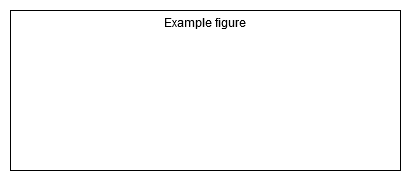
\includegraphics[width=\textwidth]{figure.png} 
    \subcaption{Source: \mycite[69]{example}}
    \label{fig:goodreference}
    \end{figure}
\blindtext

\begin{subcaptionenv}{Source: \mycite[Vgl.][2]{example}}
    \begin{lstlisting}[caption={Express Example}, language=javascript]
const express = require('express')
const app = express()
const port = 3000

app.get('/', (req, res) => res.send('Hello World!'))

app.listen(port, () => console.log(`Example app listening on port ${port}!`))
    \end{lstlisting}
\end{subcaptionenv}